\section{Pilha}

\begin{frame}[fragile]{Pilha}

    \begin{itemize}
        \item A pilha (\textit{stack}) é uma porção de memória compartilhada entre o programa e
            o sistema operacional

        \item Ela pode ser usada para a comunicação entre subprogramas, armazenamento temporário 
            e por chamadas de sistema

        \item Ela é uma estrutura LIFO (\textit{last in, first out}), isto é, o último elemento que
            foi inserido é o primeiro a ser removido

        \item Como é uma área compartilhada, ela deve ser usada com bastante cuidado, sob o risco
            de quebra do programa 

        \item O registrador \code{nasm}{ESP} (SP -- \textit{stack pointer}) contém o endereço de                memória do elemento do topo da pilha 

        \item Este registrador pode ser lido a qualquer momento, mas não pode ser escrito 
            diretamente

    \end{itemize}

\end{frame}


\begin{frame}[fragile]{Inserção de elementos na pilha}

    \begin{itemize}
        \item A instrução \code{nasm}{PUSH} insere um novo elemento no topo da pilha, atualizando
            apropriadamente o valor de \code{nasm}{ESP}

            \inputsyntax{nasm}{codes/push.st}

        \item O tamanho da memória acrescida à pilha depende do tamanho do registrador passado
            como parâmetro: 2 \textit{bytes} para um registrador de 16 \textit{bits}, 4 
            \textit{bytes} para um registrador de 32 \textit{bits}

        \item Esta instrução não suporta registradores de 8 \textit{bits}

        \item A pilha cresce ``para baixo'', isto é, um \code{nasm}{PUSH} com um registrador de
            32 \textit{bits} (por exemplo, \code{nasm}{EAX}) equivale às instruções

            \inputsyntax{nasm}{codes/push_sub.st}

    \end{itemize}

\end{frame}

\begin{frame}[fragile]{Visualização da inserção de elementos na pilha}

    \begin{figure}[ht]
        \centering
        \begin{tikzpicture}[scale=0.9]
            \node at (0.5, 5.5) { \tt 12 };
            \node at (1.5, 5.5) { \tt 34 };
            \node at (2.5, 5.5) { \tt 56 };
            \node at (3.5, 5.5) { \tt 78 };
            \node at (-0.5, 5.5) { \tt EAX };
            \draw (0, 5) rectangle (4, 6);

            \node at (2, 0.5) { \tt 28 };
            \node at (-0.5, 0.5) { \tt ESP };
            \draw (0, 0) rectangle (4, 1);

            \draw (7, 0) grid (8, 7);
            \draw (7, 0) -- (7, -0.2);
            \draw (8, 0) -- (8, -0.2);
            \draw (7, 0) -- (7, 7.2);
            \draw (8, 0) -- (8, 7.2);

            \node at (8.5, 0.5) { \tt 28 };
            \node at (8.5, 1.5) { \tt 29 };
            \node at (8.5, 2.5) { \tt 2A };
            \node at (8.5, 3.5) { \tt 2B };
            \node at (8.5, 4.5) { \tt 2C };
            \node at (8.5, 5.5) { \tt 2D };
            \node at (8.5, 6.5) { \tt 2E };
            \node at (7.5, 0.5) { \tt EF };

            \draw[->,thick] (4, 0.5) -- (7, 0.5);
        \end{tikzpicture}
        \caption{Estado do programa}
    \end{figure}

\end{frame}

\begin{frame}[fragile]{Visualização da inserção de elementos na pilha}

    \begin{figure}[ht]
        \centering
        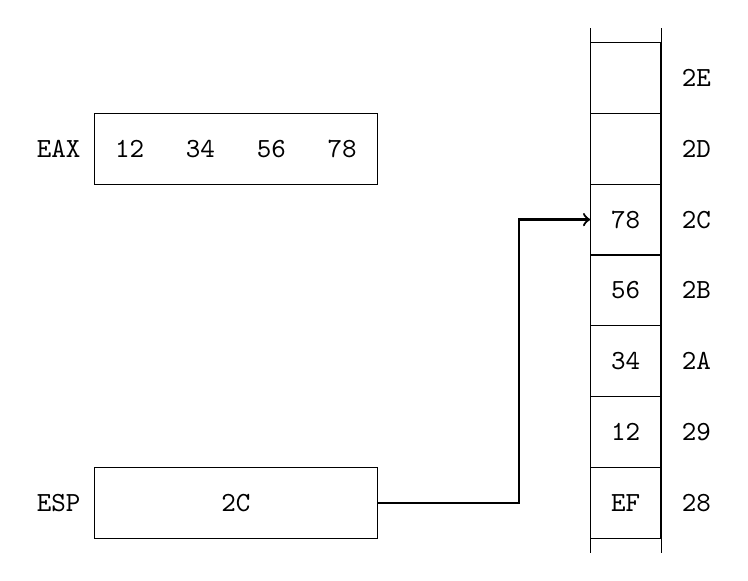
\begin{tikzpicture}[scale=0.9]
            \node at (0.5, 5.5) { \tt 12 };
            \node at (1.5, 5.5) { \tt 34 };
            \node at (2.5, 5.5) { \tt 56 };
            \node at (3.5, 5.5) { \tt 78 };
            \node at (-0.5, 5.5) { \tt EAX };
            \draw (0, 5) rectangle (4, 6);

            \node at (2, 0.5) { \tt 2C };
            \node at (-0.5, 0.5) { \tt ESP };
            \draw (0, 0) rectangle (4, 1);

            \draw (7, 0) grid (8, 7);
            \draw (7, 0) -- (7, -0.2);
            \draw (8, 0) -- (8, -0.2);
            \draw (7, 0) -- (7, 7.2);
            \draw (8, 0) -- (8, 7.2);

            \node at (8.5, 0.5) { \tt 28 };
            \node at (8.5, 1.5) { \tt 29 };
            \node at (8.5, 2.5) { \tt 2A };
            \node at (8.5, 3.5) { \tt 2B };
            \node at (8.5, 4.5) { \tt 2C };
            \node at (8.5, 5.5) { \tt 2D };
            \node at (8.5, 6.5) { \tt 2E };

            \node at (7.5, 0.5) { \tt EF };
            \node at (7.5, 1.5) { \tt 12 };
            \node at (7.5, 2.5) { \tt 34 };
            \node at (7.5, 3.5) { \tt 56 };
            \node at (7.5, 4.5) { \tt 78 };

            \draw[->,thick] (4, 0.5) -- (6, 0.5) -- (6, 4.5) -- (7, 4.5);
        \end{tikzpicture}
        \caption{Estado do programa após \code{nasm}{PUSH EAX}}
    \end{figure}

\end{frame}

\begin{frame}[fragile]{Visualização da inserção de elementos na pilha}

    \begin{figure}[ht]
        \centering
        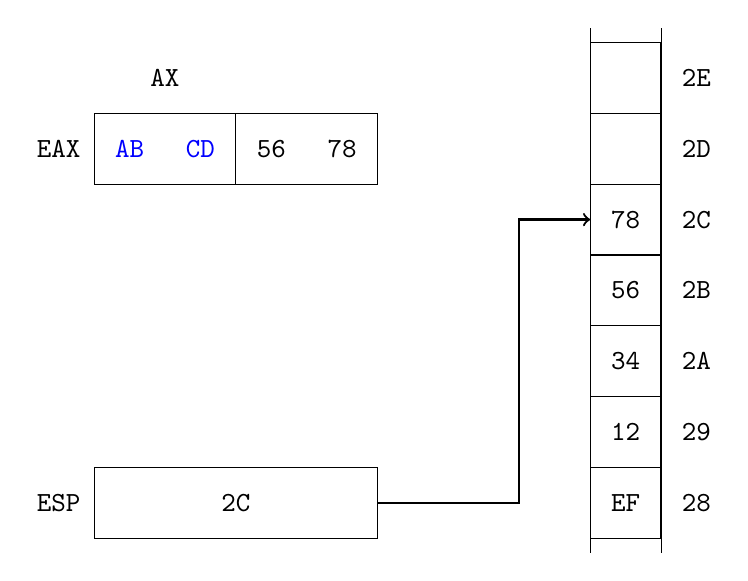
\begin{tikzpicture}[scale=0.9]
            \node at (0.5, 5.5) { \tt \textcolor{blue}{AB} };
            \node at (1.5, 5.5) { \tt \textcolor{blue}{CD} };
            \node at (2.5, 5.5) { \tt 56 };
            \node at (3.5, 5.5) { \tt 78 };
            \node at (-0.5, 5.5) { \tt EAX };
            \node at (1, 6.5) { \tt AX };
            \draw (0, 5) rectangle (2, 6);
            \draw (2, 5) rectangle (4, 6);

            \node at (2, 0.5) { \tt 2C };
            \node at (-0.5, 0.5) { \tt ESP };
            \draw (0, 0) rectangle (4, 1);

            \draw (7, 0) grid (8, 7);
            \draw (7, 0) -- (7, -0.2);
            \draw (8, 0) -- (8, -0.2);
            \draw (7, 0) -- (7, 7.2);
            \draw (8, 0) -- (8, 7.2);

            \node at (8.5, 0.5) { \tt 28 };
            \node at (8.5, 1.5) { \tt 29 };
            \node at (8.5, 2.5) { \tt 2A };
            \node at (8.5, 3.5) { \tt 2B };
            \node at (8.5, 4.5) { \tt 2C };
            \node at (8.5, 5.5) { \tt 2D };
            \node at (8.5, 6.5) { \tt 2E };

            \node at (7.5, 0.5) { \tt EF };
            \node at (7.5, 1.5) { \tt 12 };
            \node at (7.5, 2.5) { \tt 34 };
            \node at (7.5, 3.5) { \tt 56 };
            \node at (7.5, 4.5) { \tt 78 };

            \draw[->,thick] (4, 0.5) -- (6, 0.5) -- (6, 4.5) -- (7, 4.5);
        \end{tikzpicture}
        \caption{Atualização do registrador \code{nasm}{AX}}
    \end{figure}

\end{frame}

\begin{frame}[fragile]{Visualização da inserção de elementos na pilha}

    \begin{figure}[ht]
        \centering
        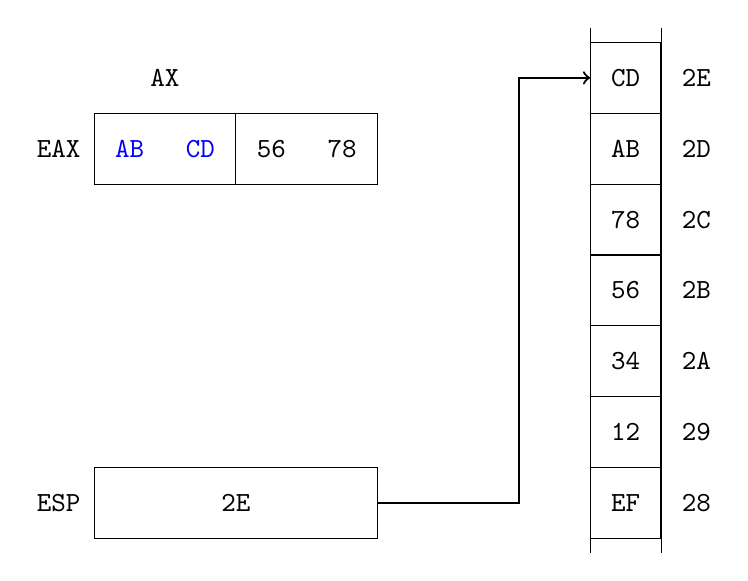
\begin{tikzpicture}[scale=0.9]
            \node at (0.5, 5.5) { \tt \textcolor{blue}{AB} };
            \node at (1.5, 5.5) { \tt \textcolor{blue}{CD} };
            \node at (2.5, 5.5) { \tt 56 };
            \node at (3.5, 5.5) { \tt 78 };
            \node at (-0.5, 5.5) { \tt EAX };
            \node at (1, 6.5) { \tt AX };
            \draw (0, 5) rectangle (2, 6);
            \draw (2, 5) rectangle (4, 6);

            \node at (2, 0.5) { \tt 2E };
            \node at (-0.5, 0.5) { \tt ESP };
            \draw (0, 0) rectangle (4, 1);

            \draw (7, 0) grid (8, 7);
            \draw (7, 0) -- (7, -0.2);
            \draw (8, 0) -- (8, -0.2);
            \draw (7, 0) -- (7, 7.2);
            \draw (8, 0) -- (8, 7.2);

            \node at (8.5, 0.5) { \tt 28 };
            \node at (8.5, 1.5) { \tt 29 };
            \node at (8.5, 2.5) { \tt 2A };
            \node at (8.5, 3.5) { \tt 2B };
            \node at (8.5, 4.5) { \tt 2C };
            \node at (8.5, 5.5) { \tt 2D };
            \node at (8.5, 6.5) { \tt 2E };

            \node at (7.5, 0.5) { \tt EF };
            \node at (7.5, 1.5) { \tt 12 };
            \node at (7.5, 2.5) { \tt 34 };
            \node at (7.5, 3.5) { \tt 56 };
            \node at (7.5, 4.5) { \tt 78 };
            \node at (7.5, 5.5) { \tt AB };
            \node at (7.5, 6.5) { \tt CD };

            \draw[->,thick] (4, 0.5) -- (6, 0.5) -- (6, 6.5) -- (7, 6.5);
        \end{tikzpicture}
        \caption{Estado do programa após \code{nasm}{PUSH AX}}
    \end{figure}

\end{frame}



\begin{frame}[fragile]{Remoção de elementos da pilha}

    \begin{itemize}
        \item A instrução \code{nasm}{POP} remove o elemento que está no topo da pilha,
            atualizando o valor de \code{nasm}{ESP} para o novo topo

            \inputsyntax{nasm}{codes/pop.st}

        \item A quantidade de \textit{bytes} que serão efetivamente removidos depende do
            tamanho do registrador passado como parâmetros: 2 \textit{bytes} para um registrador 
            de 16 \textit{bits}, 4 \textit{bytes} para um registrador de 32 \textit{bits}

        \item De forma semelhante à instrução \code{nasm}{PUSH}, não há suporte para registradores
            de 8 \textit{bits}

        \item Como a pilha cresce ``para baixo'', remover um elemento de $b$ \textit{bytes}
            equivale a somar $b$ \textit{bytes} em \code{nasm}{ESP}

        \item Assim, a instrução \code{nasm}{POP AX} equivale às instruções

            \inputsyntax{nasm}{codes/pop_add.st}
    \end{itemize}

\end{frame}

\begin{frame}[fragile]{Visualização da remoção de elementos na pilha}

    \begin{figure}[ht]
        \centering
        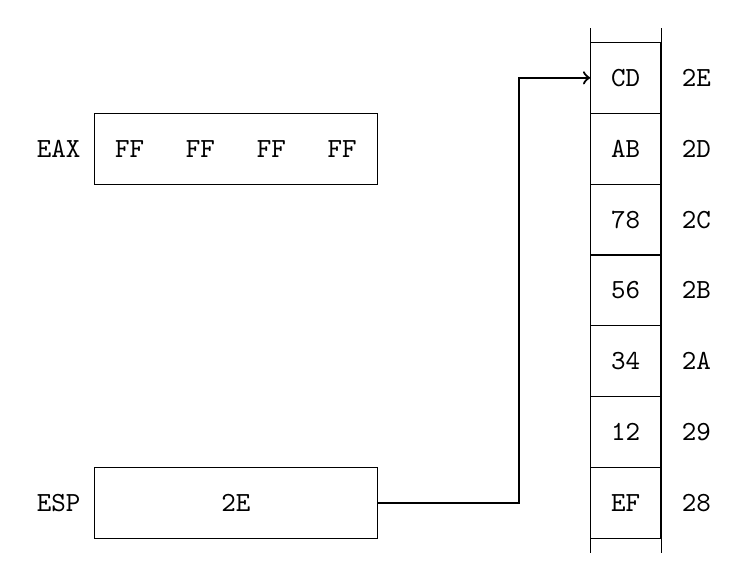
\begin{tikzpicture}[scale=0.9]
            \node at (0.5, 5.5) { \tt FF };
            \node at (1.5, 5.5) { \tt FF };
            \node at (2.5, 5.5) { \tt FF };
            \node at (3.5, 5.5) { \tt FF };
            \node at (-0.5, 5.5) { \tt EAX };
%            \node at (1, 6.5) { \tt AX };
%            \draw (0, 5) rectangle (2, 6);
            \draw (0, 5) rectangle (4, 6);

            \node at (2, 0.5) { \tt 2E };
            \node at (-0.5, 0.5) { \tt ESP };
            \draw (0, 0) rectangle (4, 1);

            \draw (7, 0) grid (8, 7);
            \draw (7, 0) -- (7, -0.2);
            \draw (8, 0) -- (8, -0.2);
            \draw (7, 0) -- (7, 7.2);
            \draw (8, 0) -- (8, 7.2);

            \node at (8.5, 0.5) { \tt 28 };
            \node at (8.5, 1.5) { \tt 29 };
            \node at (8.5, 2.5) { \tt 2A };
            \node at (8.5, 3.5) { \tt 2B };
            \node at (8.5, 4.5) { \tt 2C };
            \node at (8.5, 5.5) { \tt 2D };
            \node at (8.5, 6.5) { \tt 2E };

            \node at (7.5, 0.5) { \tt EF };
            \node at (7.5, 1.5) { \tt 12 };
            \node at (7.5, 2.5) { \tt 34 };
            \node at (7.5, 3.5) { \tt 56 };
            \node at (7.5, 4.5) { \tt 78 };
            \node at (7.5, 5.5) { \tt AB };
            \node at (7.5, 6.5) { \tt CD };

            \draw[->,thick] (4, 0.5) -- (6, 0.5) -- (6, 6.5) -- (7, 6.5);
        \end{tikzpicture}
        \caption{Estado do programa}
    \end{figure}

\end{frame}

\begin{frame}[fragile]{Visualização da remoção de elementos na pilha}

    \begin{figure}[ht]
        \centering
        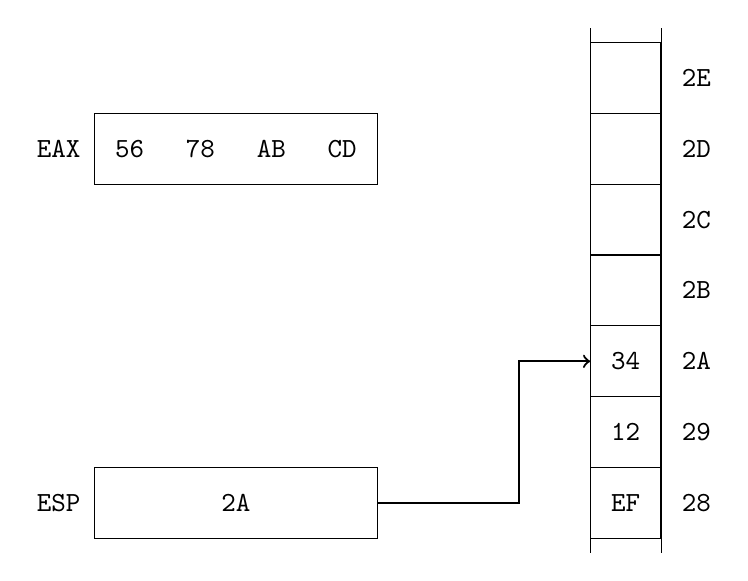
\begin{tikzpicture}[scale=0.9]
            \node at (0.5, 5.5) { \tt 56 };
            \node at (1.5, 5.5) { \tt 78 };
            \node at (2.5, 5.5) { \tt AB };
            \node at (3.5, 5.5) { \tt CD };
            \node at (-0.5, 5.5) { \tt EAX };
%            \node at (1, 6.5) { \tt AX };
%            \draw (0, 5) rectangle (2, 6);
            \draw (0, 5) rectangle (4, 6);

            \node at (2, 0.5) { \tt 2A };
            \node at (-0.5, 0.5) { \tt ESP };
            \draw (0, 0) rectangle (4, 1);

            \draw (7, 0) grid (8, 7);
            \draw (7, 0) -- (7, -0.2);
            \draw (8, 0) -- (8, -0.2);
            \draw (7, 0) -- (7, 7.2);
            \draw (8, 0) -- (8, 7.2);

            \node at (8.5, 0.5) { \tt 28 };
            \node at (8.5, 1.5) { \tt 29 };
            \node at (8.5, 2.5) { \tt 2A };
            \node at (8.5, 3.5) { \tt 2B };
            \node at (8.5, 4.5) { \tt 2C };
            \node at (8.5, 5.5) { \tt 2D };
            \node at (8.5, 6.5) { \tt 2E };

            \node at (7.5, 0.5) { \tt EF };
            \node at (7.5, 1.5) { \tt 12 };
            \node at (7.5, 2.5) { \tt 34 };
%            \node at (7.5, 3.5) { \tt 56 };
%            \node at (7.5, 4.5) { \tt 78 };
%            \node at (7.5, 5.5) { \tt AB };
%            \node at (7.5, 6.5) { \tt CD };

            \draw[->,thick] (4, 0.5) -- (6, 0.5) -- (6, 2.5) -- (7, 2.5);
        \end{tikzpicture}
        \caption{Estado do programa após a instrução \code{nasm}{POP EAX}}
    \end{figure}

\end{frame}



\begin{frame}[fragile]{Exemplo de uso da pilha}
    \inputsnippet{nasm}{1}{22}{codes/print_int.s}
\end{frame}

\begin{frame}[fragile]{Exemplo de uso da pilha}
    \inputsnippet{nasm}{23}{44}{codes/print_int.s}
\end{frame}

\begin{frame}[fragile]{Exemplo de uso da pilha}
    \inputsnippet{nasm}{45}{57}{codes/print_int.s}
\end{frame}
